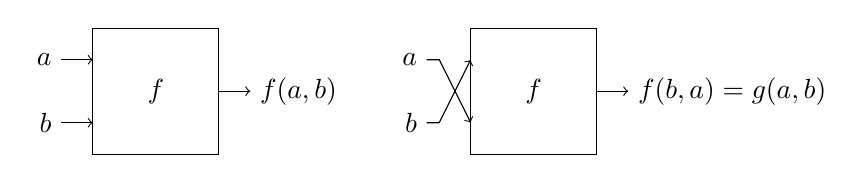
\begin{tikzpicture}[scale=0.8]

\draw (1,0) rectangle (3,2);
\node at (2,1)  {$f$};
\draw [->] (3,1) -- (3.5,1) node [right] {$f(a,b)$};
\draw [->] (0.5,1.5) node [left] {$a$} -- (1,1.5);
\draw [->] (0.5,0.5) node [left] {$b$} -- (1,0.5);

\draw (7,0) rectangle (9,2);
\node at (8,1)  {$f$};
\draw [->] (9,1) -- (9.5,1) node [right] {$f(b,a) = g(a,b)$};
\draw [->] (6.3,1.5) node [left] {$a$} -- (6.5,1.5) -- (7,0.5);
\draw [->] (6.3,0.5) node [left] {$b$} -- (6.5,0.5) -- (7,1.5);

\end{tikzpicture}
